% Appendix

\section{Rubric Text}
\label{app:rubric}

\subsection{Conditions 2 and 3 (Likert Scale)}

The following text is appended to the agent's prompt when skills are retrieved and injected:

\begin{quote}
\small\ttfamily\raggedright\noindent
RETRIEVAL FEEDBACK --- MANDATORY (if skills were provided above):\\{}
[RETRIEVAL EFFECTIVENESS]\\{}
You were provided with skills retrieved using three scoring dimensions:\\{}
- RECENCY: How recent/fresh the skill is\\{}
- IMPORTANCE: How important it was previously flagged\\{}
- RELEVANCE: How well it semantically matches your current task\\[\medskipamount]
Rate how useful EACH dimension was for helping you complete this specific task.\\{}
You MUST use exactly this format (one rating per line, number only):\\[\medskipamount]
Recency: <single number 1-5, where 1=irrelevant to task, 5=essential>\\{}
Importance: <single number 1-5>\\{}
Relevance: <single number 1-5>\\[\medskipamount]
Brief explanation (2-3 sentences):\\{}
- Which dimension was most valuable and why?\\{}
- Which dimension was least valuable and why?\\{}
- What KIND of skills would have been even more helpful?\\{}
[/RETRIEVAL EFFECTIVENESS]
\end{quote}

\subsection{Condition 4 (Qualitative, Separated Questions)}

\begin{quote}
\small\ttfamily\raggedright\noindent
RETRIEVAL FEEDBACK --- MANDATORY (if skills were provided above):\\{}
[RETRIEVAL EFFECTIVENESS]\\{}
Evaluate how useful each retrieval dimension was for this specific task.\\{}
You MUST respond inside each tagged section below with 2-3 sentences.\\[\medskipamount]
[RECENCY EVALUATION]\\{}
How important was the freshness/timing of the retrieved skills for this task?\\{}
Were recently-used skills more helpful than older ones, or did timing not matter?\\{}
[/RECENCY EVALUATION]\\[\medskipamount]
[IMPORTANCE EVALUATION]\\{}
How important was the proven track record of the retrieved skills for this task?\\{}
Did you need battle-tested, reliable skills, or would untested ones have worked?\\{}
[/IMPORTANCE EVALUATION]\\[\medskipamount]
[RELEVANCE EVALUATION]\\{}
How important was the subject matter match of the retrieved skills for this task?\\{}
Were topically aligned skills essential, or could off-topic skills have helped?\\{}
[/RELEVANCE EVALUATION]\\{}
[/RETRIEVAL EFFECTIVENESS]
\end{quote}

\section{Anchor Embedding Design}
\label{app:anchors}

Table~\ref{tab:anchors} summarizes the calibration results for the separated-question anchor parser (Condition~4).
Anchors describe qualitatively different scenarios rather than degree variations to maximize embedding distance.

The anchor texts for each dimension are:

\paragraph{Recency anchors.}
\textbf{Low:} ``I already knew the current state of the art for this task. The retrieved skills, whether old or new, were redundant---freshness made no difference because the fundamentals haven't changed.''
\textbf{Mid:} ``I used a standard approach that has been around for a while. Recently used skills gave me useful context for incremental improvements, but I could have solved it with older knowledge alone.''
\textbf{High:} ``This task required cutting-edge techniques that have only emerged recently. Only the most recently practiced skills had methods I wasn't already familiar with. Older skills were obsolete.''

\paragraph{Importance anchors.}
\textbf{Low:} ``I solved this task from first principles and experimentation. Whether the skills had been successfully applied before didn't affect my approach---I would have tried any method regardless of track record.''
\textbf{Mid:} ``Proven skills gave me more confidence in my approach, but I would have still explored unproven alternatives if needed. Track record was a useful signal but not decisive.''
\textbf{High:} ``This task was too high-stakes to experiment with unproven methods. I relied exclusively on skills with demonstrated success because failure would have been costly. Untested approaches were unacceptable.''

\paragraph{Relevance anchors.}
\textbf{Low:} ``I needed creative cross-domain thinking for this task. Skills from unrelated fields sparked novel ideas just as much as on-topic skills. Semantic match to the task description was irrelevant.''
\textbf{Mid:} ``I needed a mix of deep domain knowledge and lateral thinking. On-topic skills provided essential structure, but insights from adjacent fields also contributed meaningfully to my solution.''
\textbf{High:} ``This task demanded deep, specialized domain expertise. Only skills directly about the exact topic were useful---off-topic skills were noise that distracted from the precise technical requirements.''

\begin{table}[t]
\centering
\small
\begin{tabular}{lccccc}
\toprule
\textbf{Dim.} & \textbf{Low} & \textbf{Mid} & \textbf{High} & \textbf{Spread} & \textbf{Order} \\
\midrule
Recency & 0.175 & 0.409 & 0.745 & 0.570 & \checkmark \\
Importance & 0.207 & 0.542 & 0.924 & 0.717 & \checkmark \\
Relevance & 0.162 & 0.344 & 0.822 & 0.660 & \checkmark \\
\bottomrule
\end{tabular}
\caption{Anchor calibration results ($\tau=0.05$, 9 synthetic texts per dimension). Spread $=$ high $-$ low. Order preserved (low $<$ mid $<$ high) across all 27 test texts.}
\label{tab:anchors}
\end{table}

\section{Skill Library Design}
\label{app:skills}

\paragraph{Experiment 1 (v2).}
50 meta-skills across 5 domains: research (10), creative (10), synthesis (10), evaluation (10), operational (10).
Skills are procedural and domain-general (e.g., ``Systematic Literature Review,'' ``Hypothesis Generation Framework'').

\paragraph{Experiment 2 (v3).}
205 domain-specific skills: 30 base skills plus 175 specialized skills distributed across 5 themes (${\sim}$35 per theme: ML Fundamentals, Agent Architectures, Multi-Agent Systems, Evaluation Methods, Retrieval Systems).
Specialized skills are designed to be relevant to specific task types within each theme, ensuring that weight configurations can produce different top-5 retrievals.

\section{Task Corpus Construction}
\label{app:tasks}

\paragraph{Experiment 1 (v2).}
250 tasks: 100 easy, 100 medium, 50 hard.
Tasks are distributed across 5 themes (50 per theme).
Difficulty is determined by expected reasoning depth: easy tasks require single-step retrieval, medium tasks require integration of 2--3 skills, hard tasks require multi-step reasoning or cross-domain synthesis.

\paragraph{Experiment 2 (v3).}
300 tasks: 50 easy, 100 medium, 150 hard.
The shift toward harder tasks increases the expected impact of retrieval quality on performance.
Ground truth skill annotations (1--3 relevant skills per task) enable measurement of retrieval precision via ground truth hit rate.

\section{Thompson Sampling vs.\ UCB}
\label{app:ts_vs_ucb}

We chose Thompson Sampling (TS) over Upper Confidence Bound (UCB) variants for four reasons specific to our problem setting.

\paragraph{Stochastic rewards from noisy self-assessment.}
LLM dimension ratings are inherently noisy: the same retrieval configuration applied to similar tasks produces reward variance of 0.15--0.25 across episodes.
TS models this naturally via Beta posteriors: uncertainty is represented probabilistically, and exploration is driven by posterior width rather than a manually tuned confidence bound.
UCB1 computes $\bar{x}_k + c\sqrt{\ln t / n_k}$, requiring selection of the exploration constant $c$.
In our setting, reward noise is non-uniform across arms (presets that emphasize relevance have lower variance than balanced presets), making a single $c$ suboptimal.
TS adapts to per-arm variance without tuning.

\paragraph{Exploration without hyperparameters.}
$\epsilon$-greedy and UCB both require exploration parameters ($\epsilon$, $c$) that affect convergence speed and final regret.
TS draws directly from the posterior: wide posteriors produce high-variance samples (exploration), and narrow posteriors produce concentrated samples (exploitation).
This property is especially valuable when the number of episodes per condition is fixed by experimental budget (250--300), so there is no opportunity to tune exploration parameters via a validation split.

\paragraph{Finite-arm optimality.}
With $K \in \{5, 12\}$ discrete weight presets, TS achieves the Lai--Robbins lower bound on asymptotic regret for Bernoulli rewards~\citep{agrawal2012analysis}; with our continuous pseudo-count updates, the bound is approximate but convergence behavior is preserved in practice.
We deliberately keep the action space discrete (presets on the weight simplex) rather than attempting continuous optimization, because: (a) the reward signal is too noisy for gradient estimation, (b) the simplex constraint complicates continuous bandit methods, and (c) 5--12 presets provide sufficient coverage of qualitatively different retrieval strategies.

\paragraph{Compatibility with non-stationarity.}
While our experimental design is stationary (tasks are shuffled), a production deployment would face concept drift as the skill library evolves.
TS with discounted posteriors (multiplying $\alpha_k, \beta_k$ by a decay factor each episode) handles non-stationarity gracefully, whereas UCB confidence bounds must be explicitly re-calibrated.
We do not use discounting in the controlled experiment, but the architecture supports it.

\paragraph{Empirical validation.}
We verified the choice empirically using data from both experiments (1{,}000 v2 episodes and 1{,}200 v3 episodes).
Cumulative regret was computed against an oracle that always selects the highest-reward arm.
Across conditions C2--C4, TS regret is sublinear and stabilizes by episode 100--150 (see Figure~\ref{fig:convergence_curves} for posterior trajectories and Figure~\ref{fig:cumulative_regret} for cumulative regret), consistent with the theoretical $O(\sqrt{KT \ln T})$ bound.
In v3, C3 converges to \texttt{pure\_relevance} with posterior mean 0.749 by approximately episode 44, demonstrating rapid lock-in when the reward signal is informative.

\section{Statistical Methods}
\label{app:stats}

All primary comparisons use bootstrap confidence intervals (10,000 resamples) rather than parametric tests, due to extreme variance heterogeneity across conditions (C1 SD$=$24{,}746 vs.\ C4 SD$=$2{,}037 in v2; C1 SD$=$2{,}449 vs.\ C4 SD$=$1{,}429 in v3).
We report two-sided bootstrap $p$-values computed as the fraction of resamples where the difference crosses zero.
For v3, we additionally report Kruskal--Wallis omnibus tests (non-parametric), Mann--Whitney $U$ for pairwise comparisons with Holm--Bonferroni correction (six comparisons), and Cohen's $d$ effect sizes.
Effect sizes are reported as percentage reduction in mean token consumption relative to C1.

\section{Supplementary Figures}
\label{app:figures}

\begin{figure}[t]
\centering
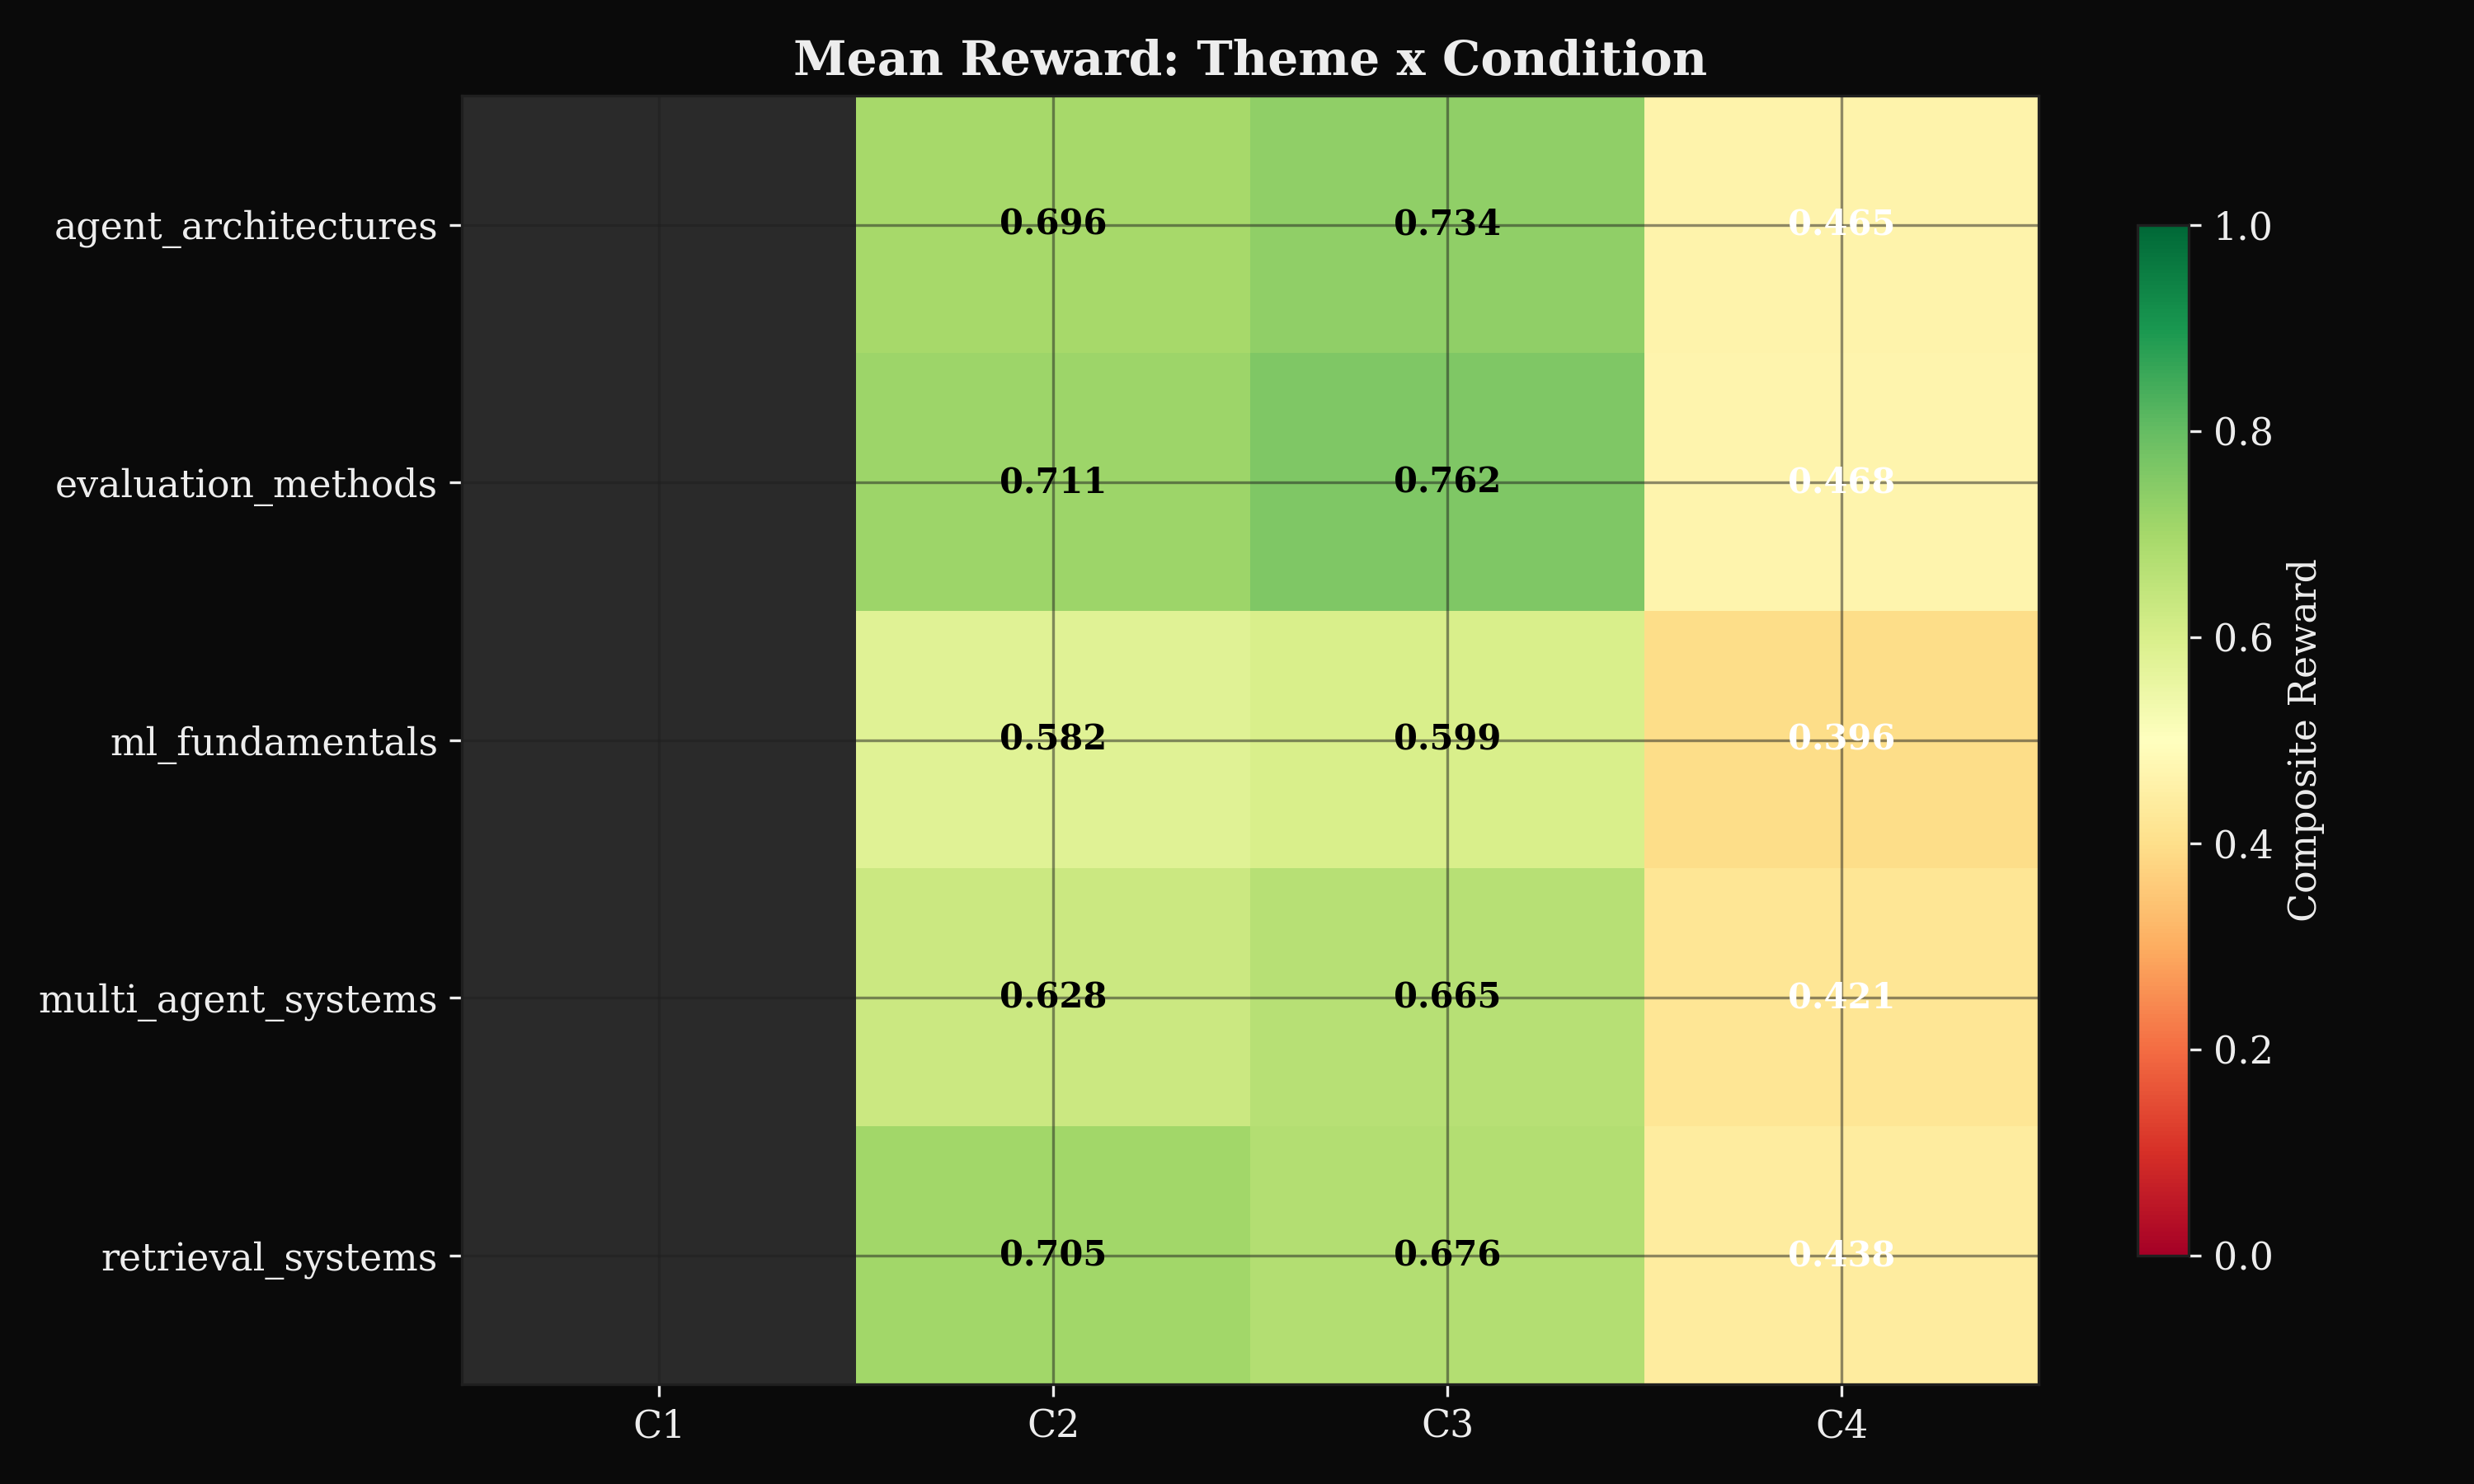
\includegraphics[width=\columnwidth]{../results/figures/fig3_theme_heatmap.png}
\caption{Mean reward by condition and theme. Reward variation across themes is modest ($<$0.15 range), consistent with the rubric prompt effect dominating over theme-specific retrieval differences.}
\label{fig:theme_heatmap}
\end{figure}

\begin{figure}[t]
\centering
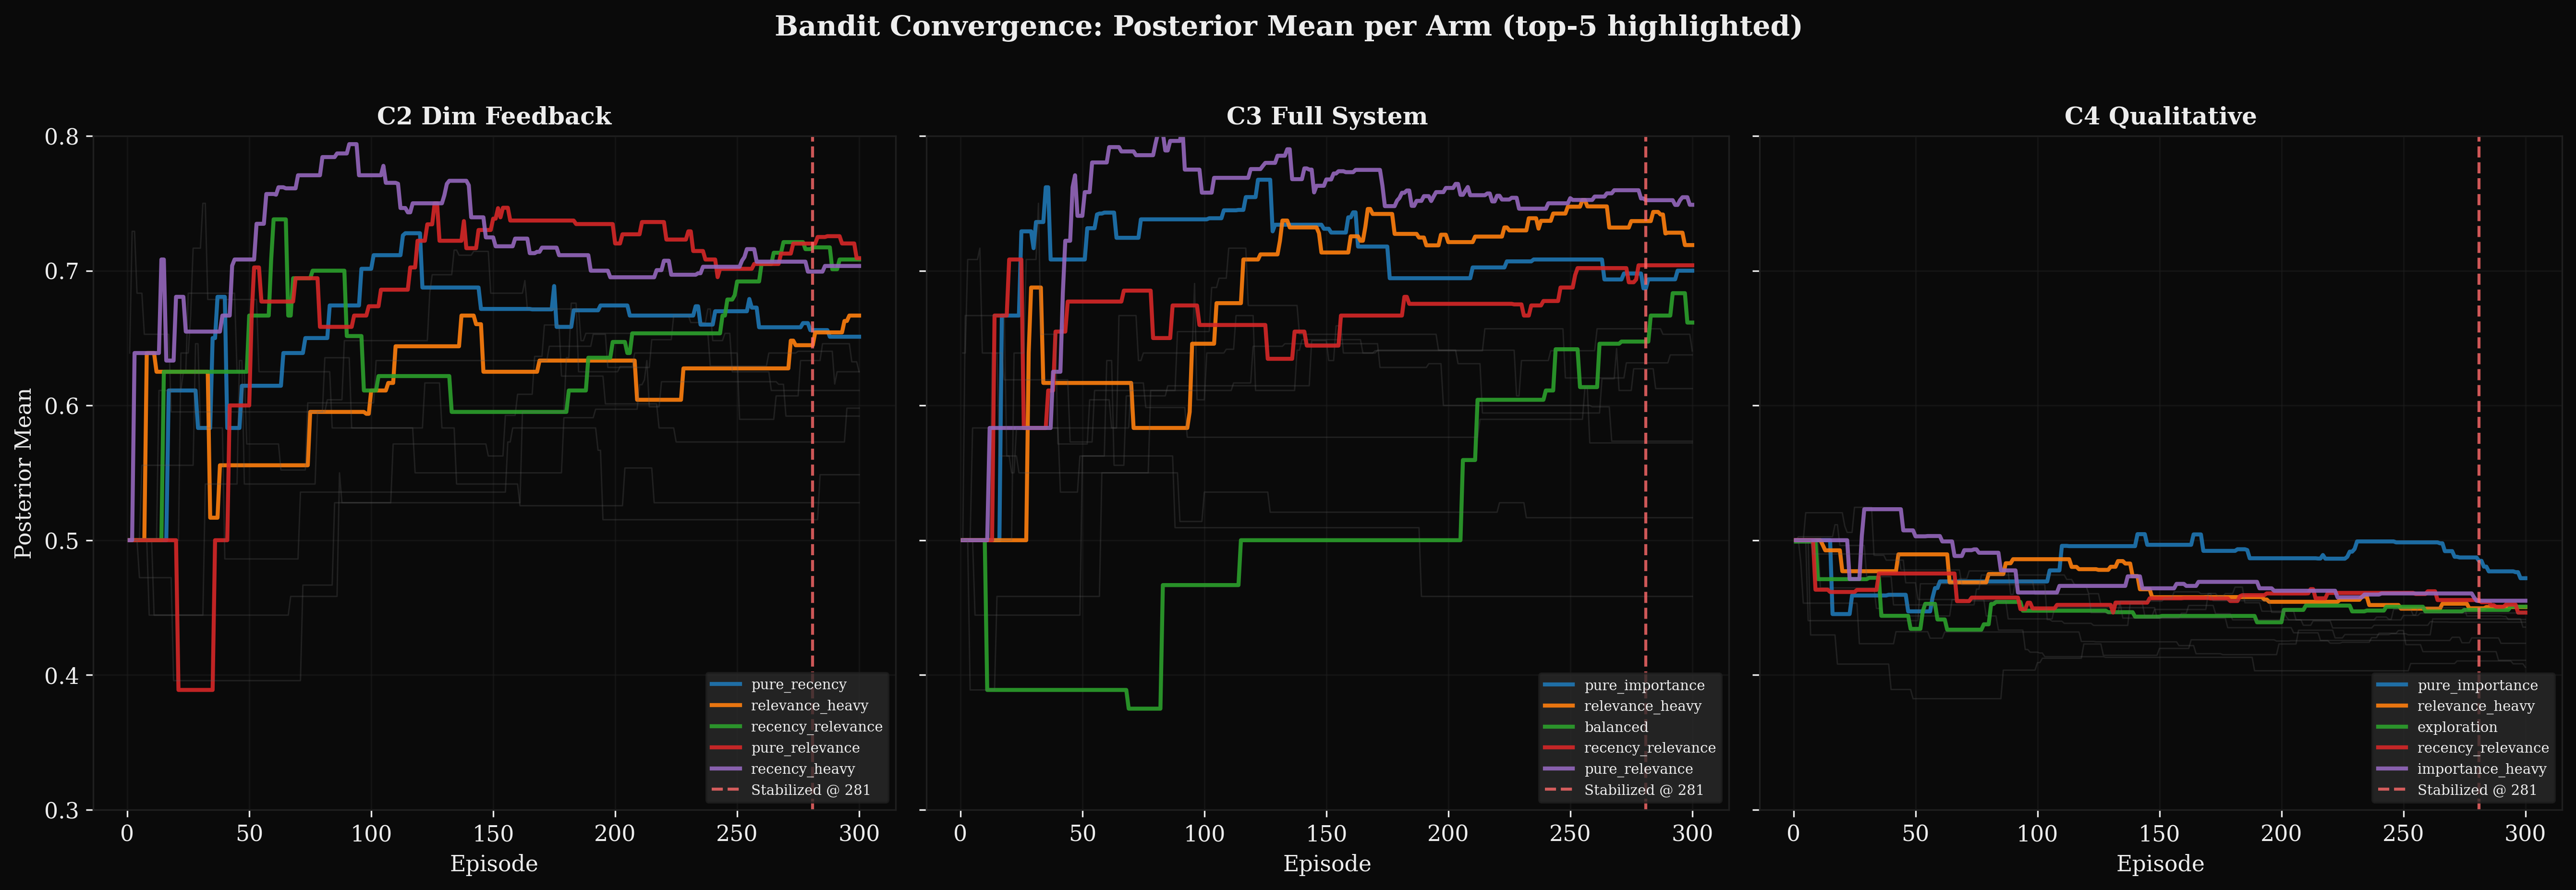
\includegraphics[width=\columnwidth]{../results/figures/fig2_convergence_curves.png}
\caption{Thompson Sampling posterior mean trajectories over episodes (v3, 12 arms, top 5 highlighted). C2 and C3 both converge toward \texttt{pure\_relevance}; C3 reaches a stable selection pattern by task 33--48. C4 shows compressed posteriors with all arms near 0.45, reflecting the anchor parser's limited discriminative signal.}
\label{fig:convergence_curves}
\end{figure}

\begin{figure}[t]
\centering
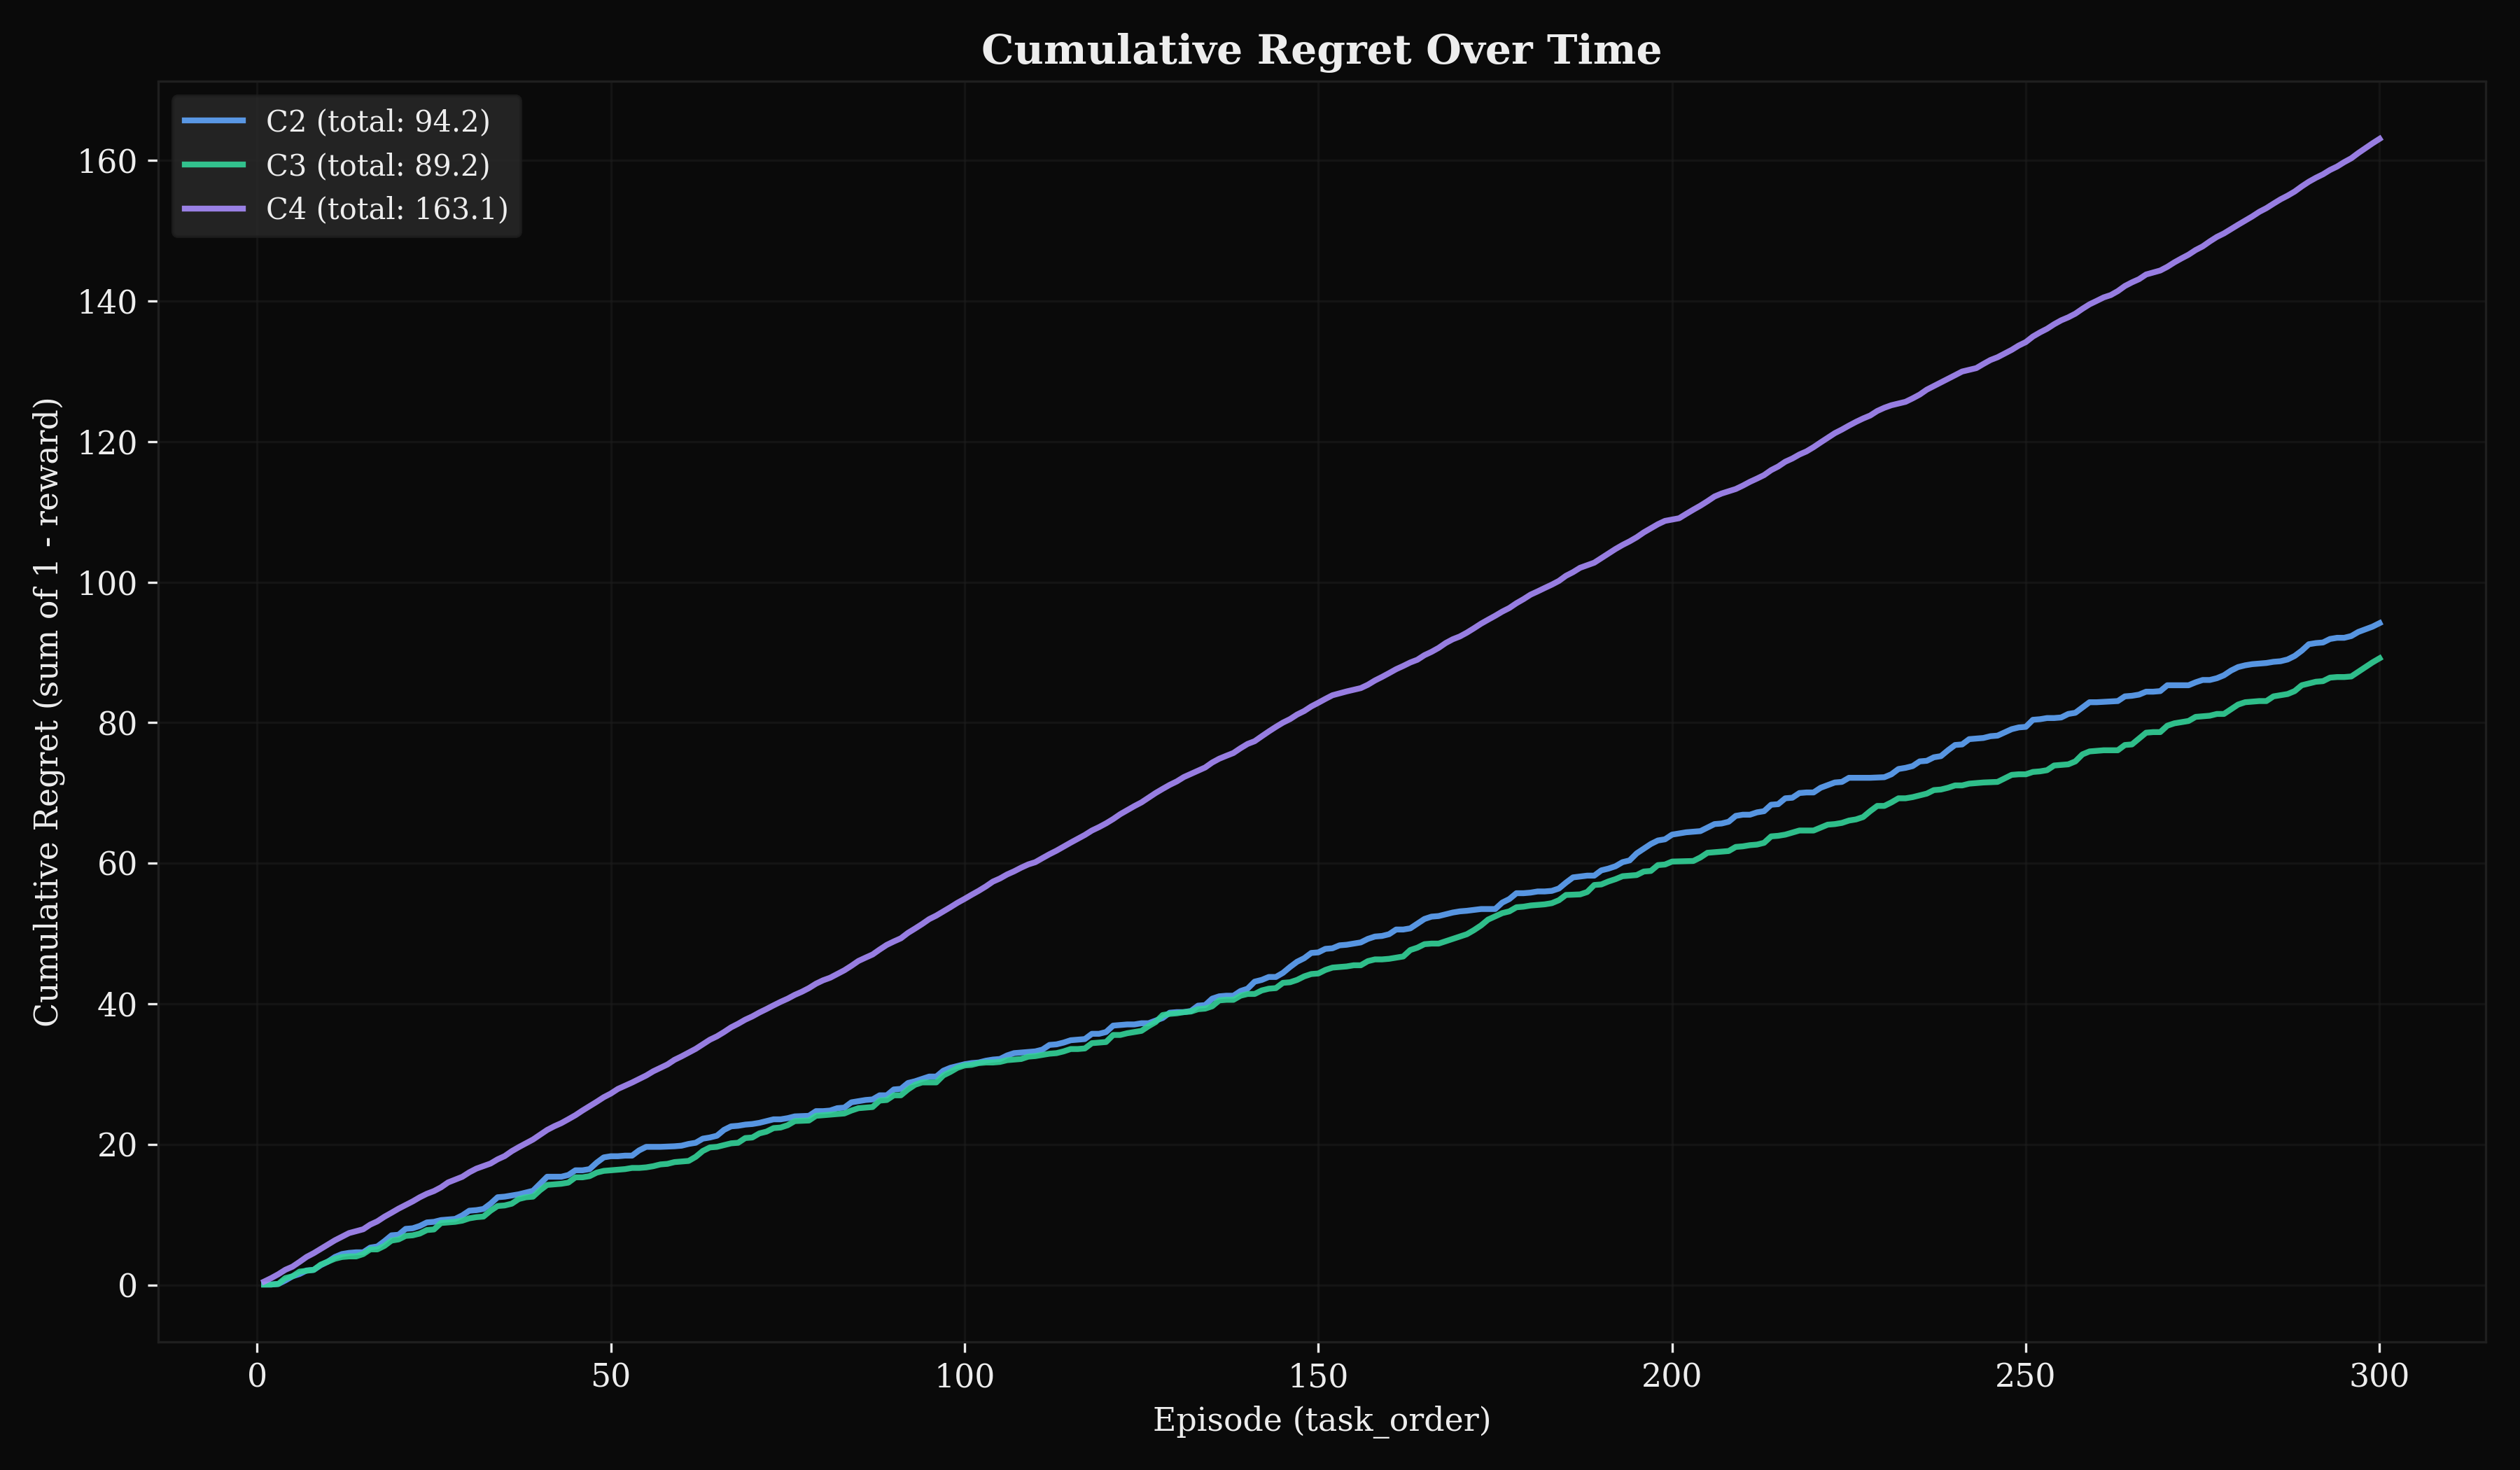
\includegraphics[width=\columnwidth]{../results/figures/fig5_cumulative_regret.png}
\caption{Cumulative regret for Thompson Sampling in C2, C3, and C4. Regret is computed against an oracle that always selects the highest-reward arm. C2 and C3 show sublinear regret growth consistent with convergence; C4's linear regret reflects compressed reward variance preventing arm differentiation.}
\label{fig:cumulative_regret}
\end{figure}

% fig7_jaccard_trajectory.png is now included in experiment_v3.tex (Figure~\ref{fig:v3_jaccard_trajectory})
% with a caption covering both v2 and v3 data. Removed duplicate here.

\begin{figure}[t]
\centering
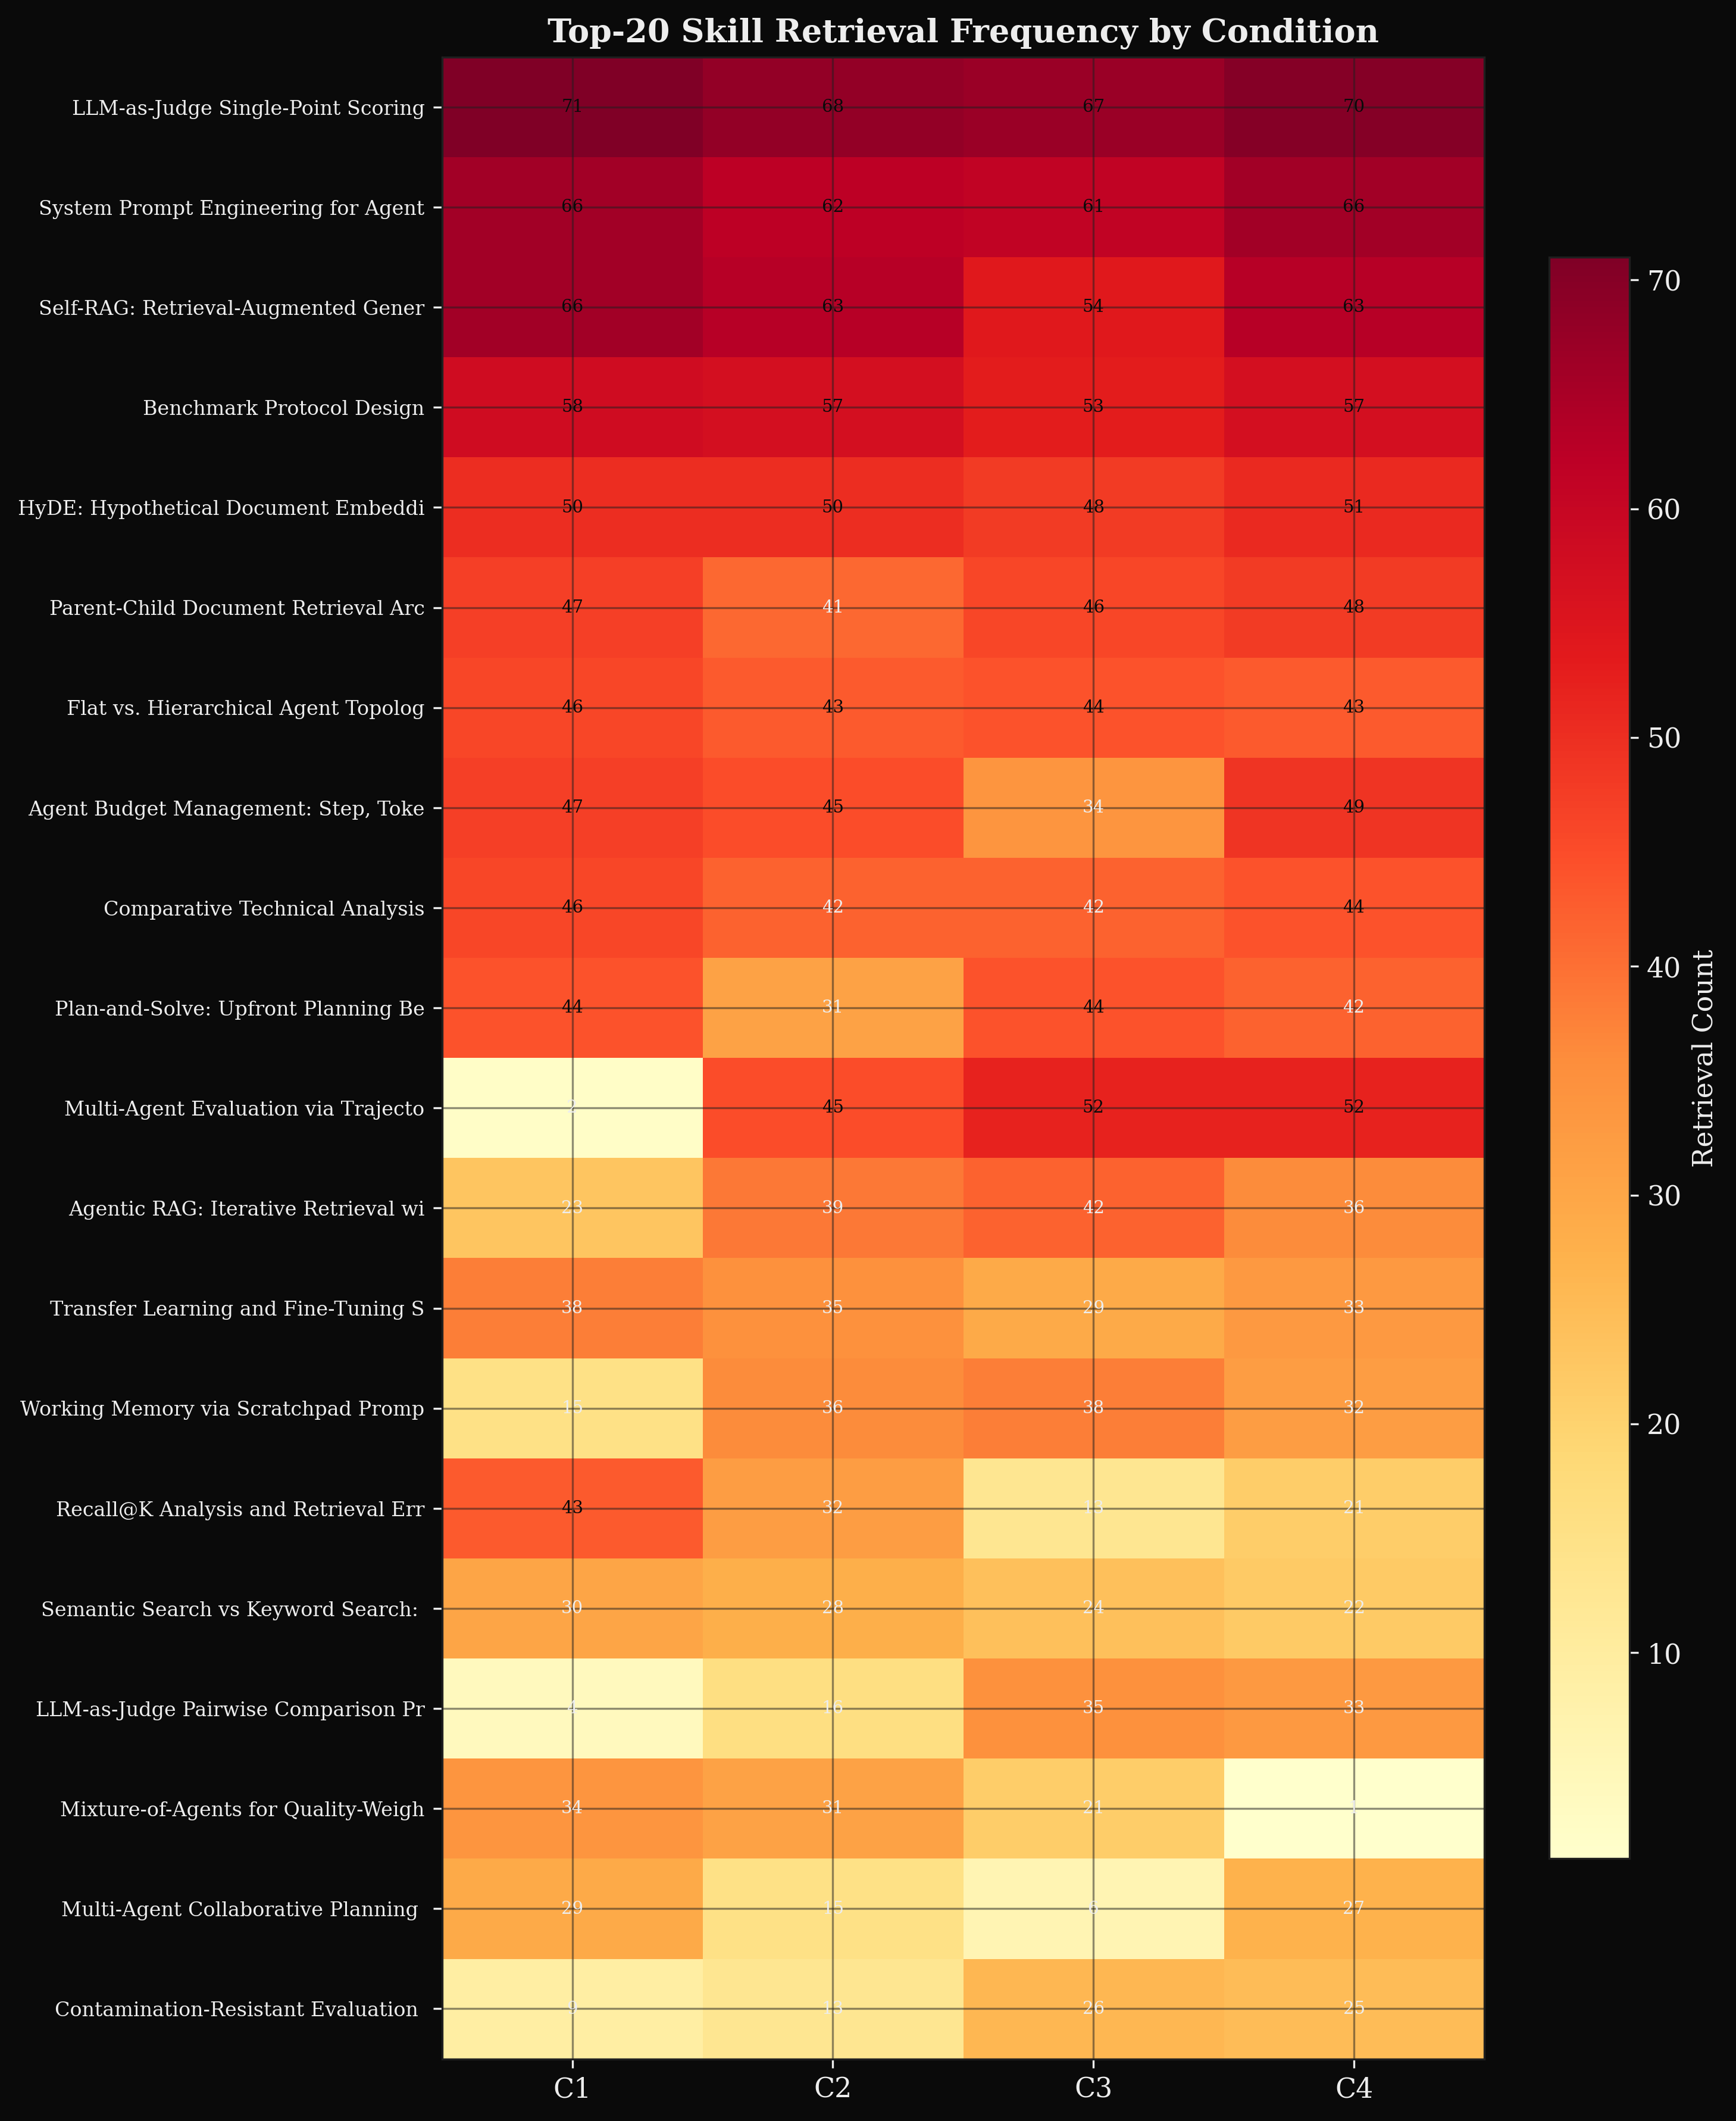
\includegraphics[width=\columnwidth]{../results/figures/figA1_skill_retrieval_heatmap.png}
\caption{Skill retrieval frequency heatmap. A small number of generic skills dominate retrieval across all conditions, explaining why weight changes do not change the top-5 set.}
\label{fig:skill_heatmap}
\end{figure}

\begin{figure}[t]
\centering
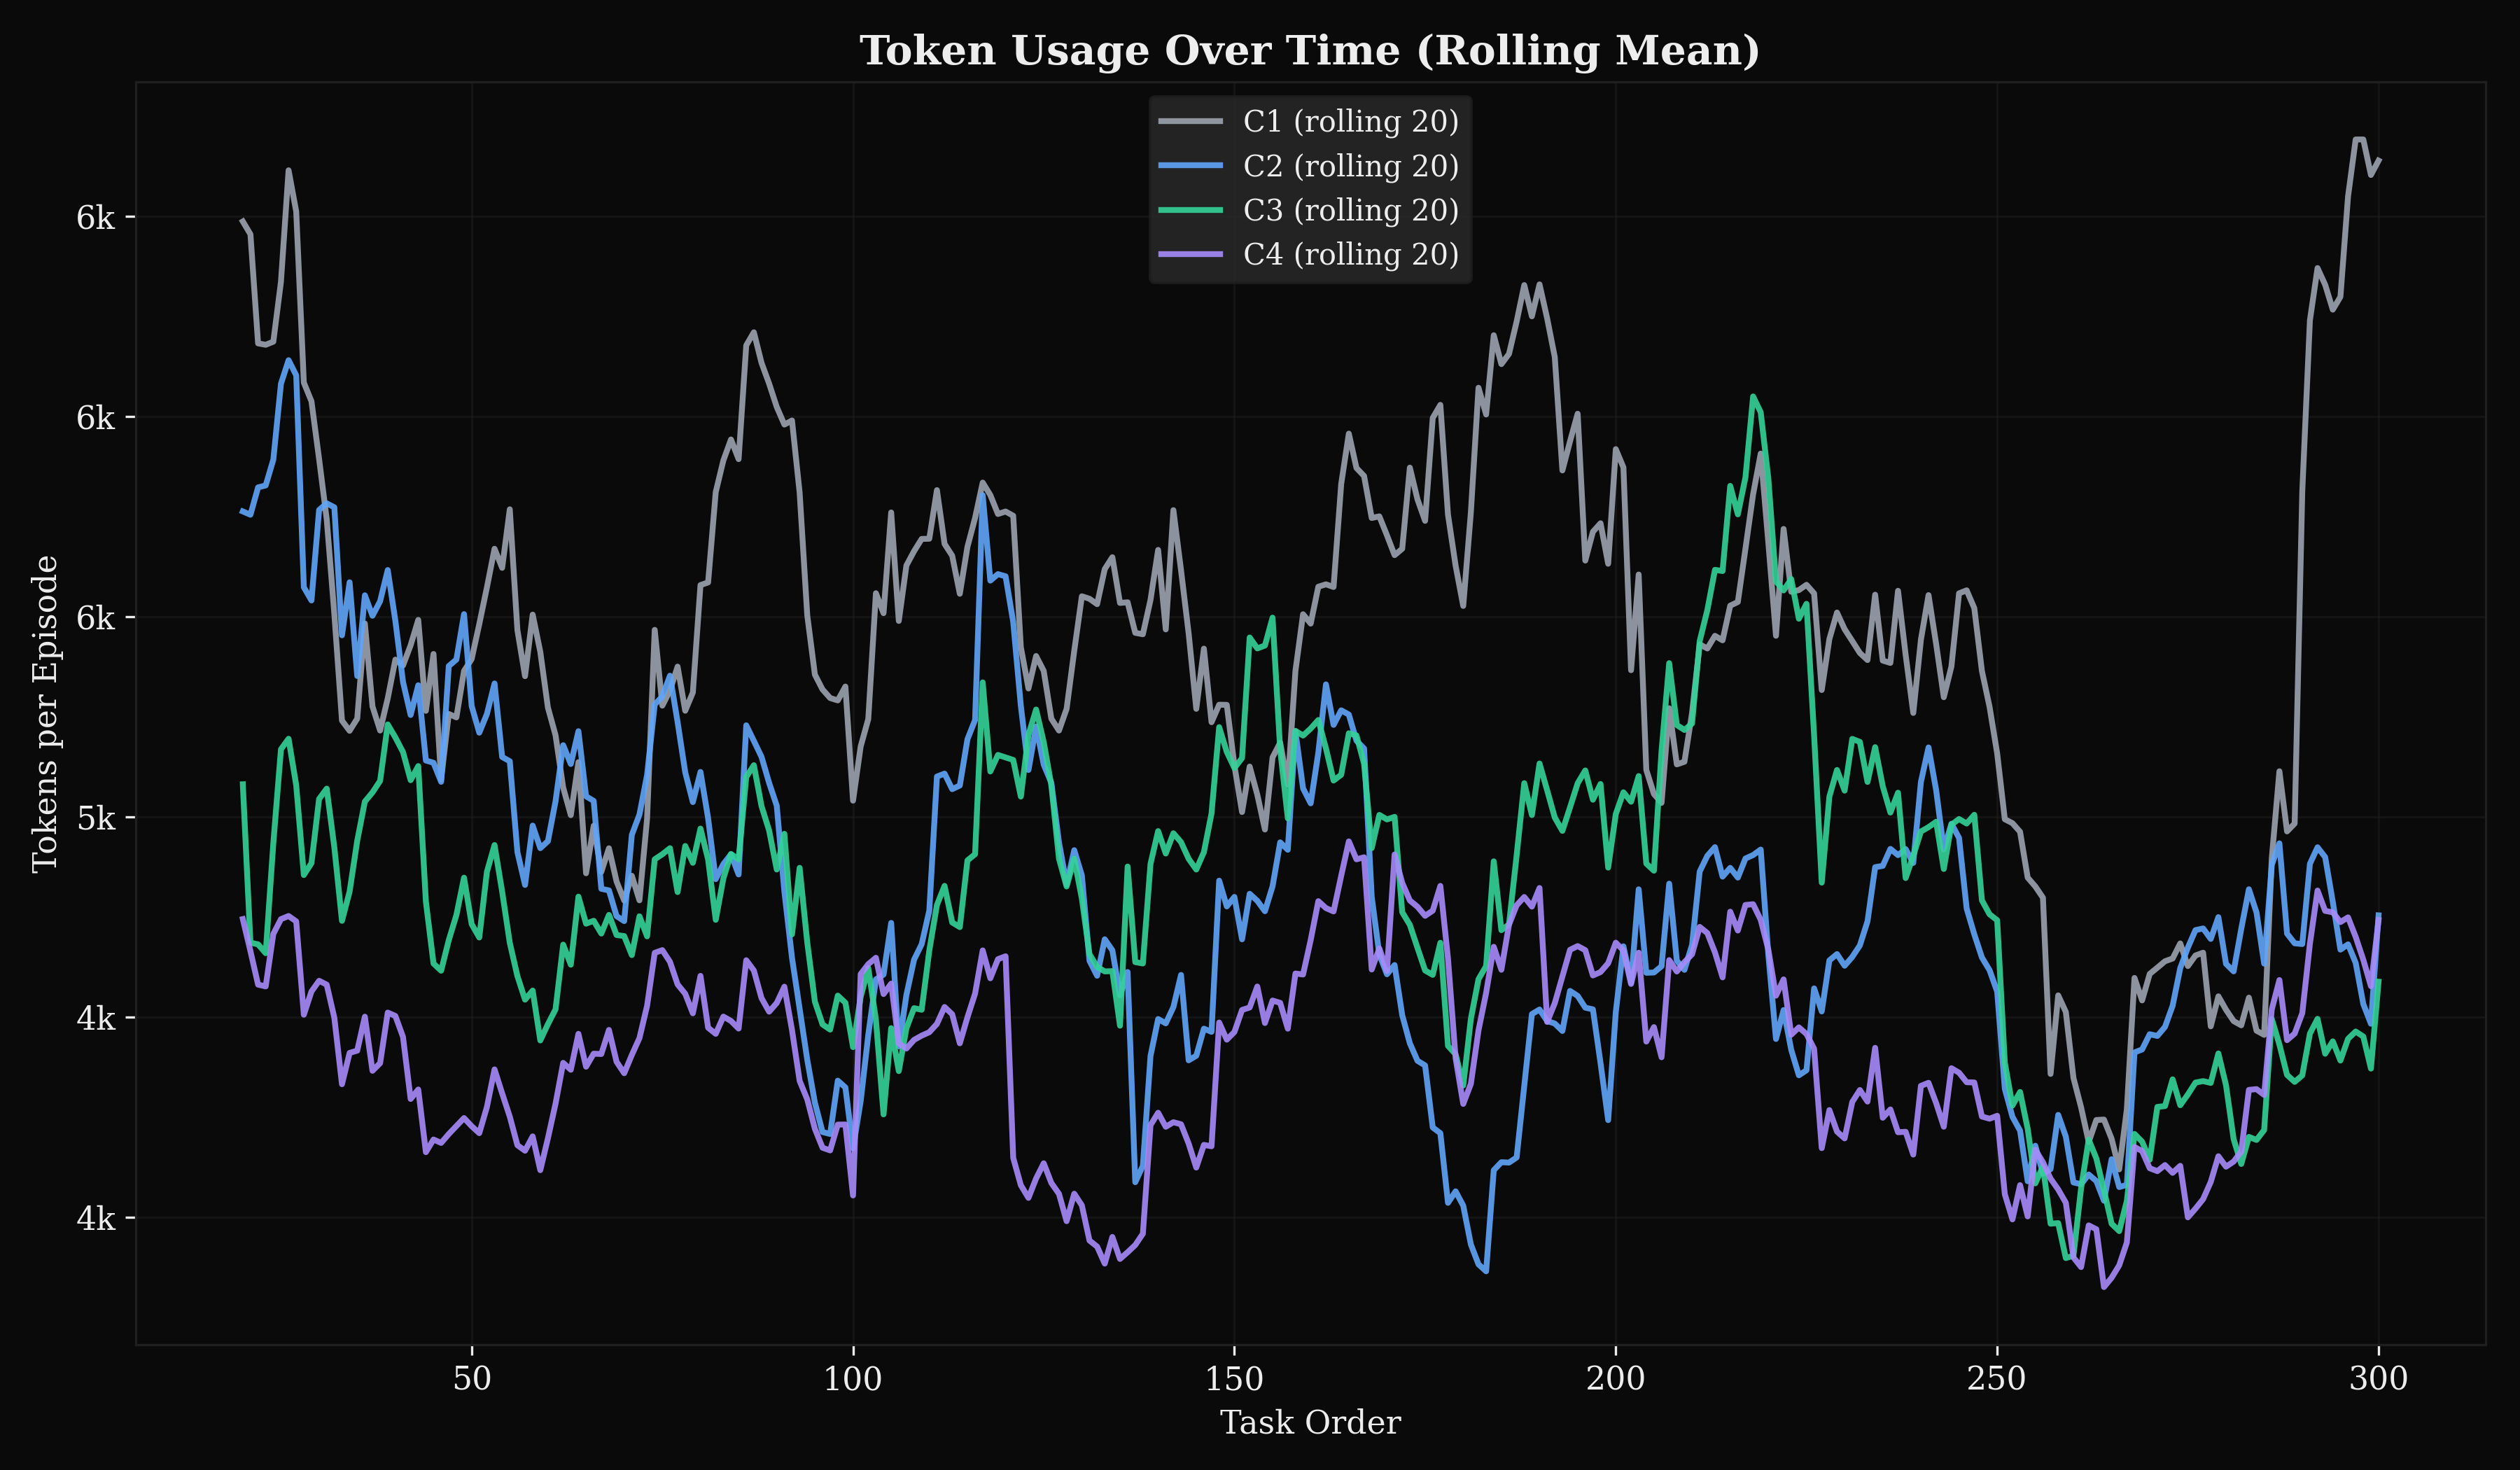
\includegraphics[width=\columnwidth]{../results/figures/figA2_token_trend.png}
\caption{Token consumption trend over episodes. No systematic drift is visible, confirming the absence of in-context learning effects or reward hacking.}
\label{fig:token_trend}
\end{figure}

\begin{figure}[t]
\centering
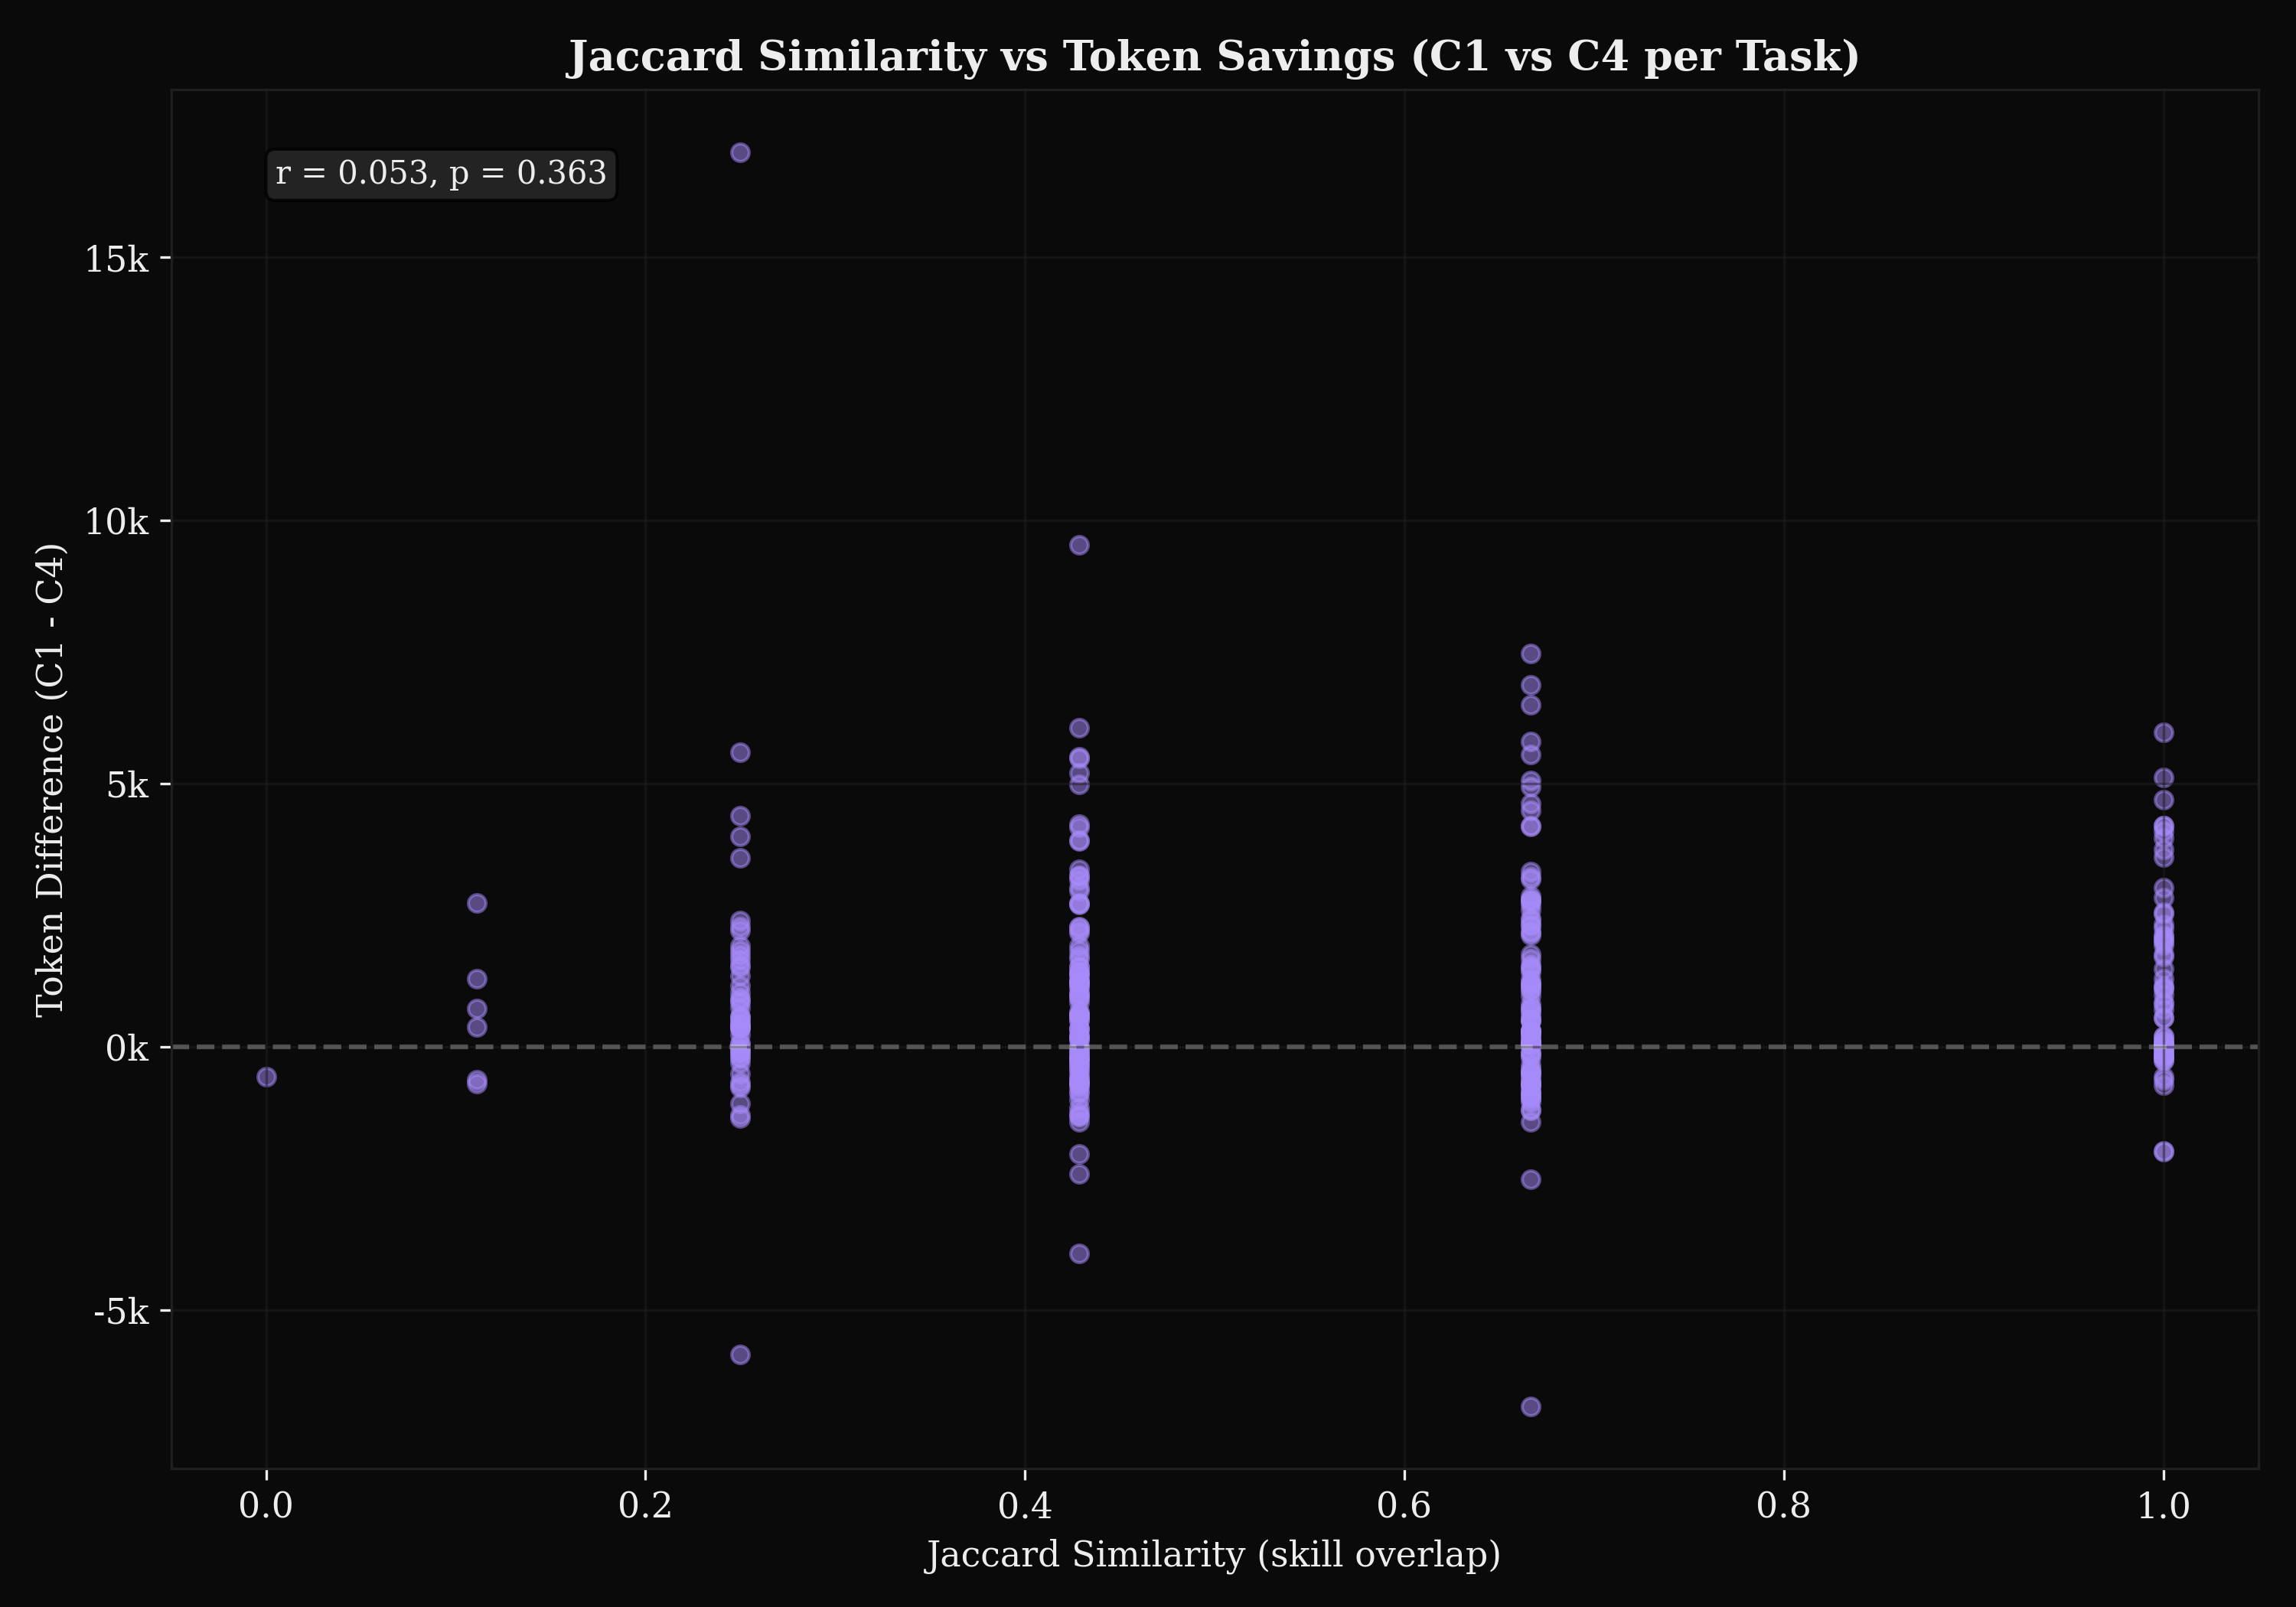
\includegraphics[width=\columnwidth]{../results/figures/figA4_jaccard_vs_tokens.png}
\caption{Relationship between Jaccard overlap and token consumption. Higher overlap (more similar retrievals) does not correlate with higher tokens, confirming that retrieval content is not the driver of token variation.}
\label{fig:jaccard_vs_tokens}
\end{figure}

\begin{figure}[t]
\centering
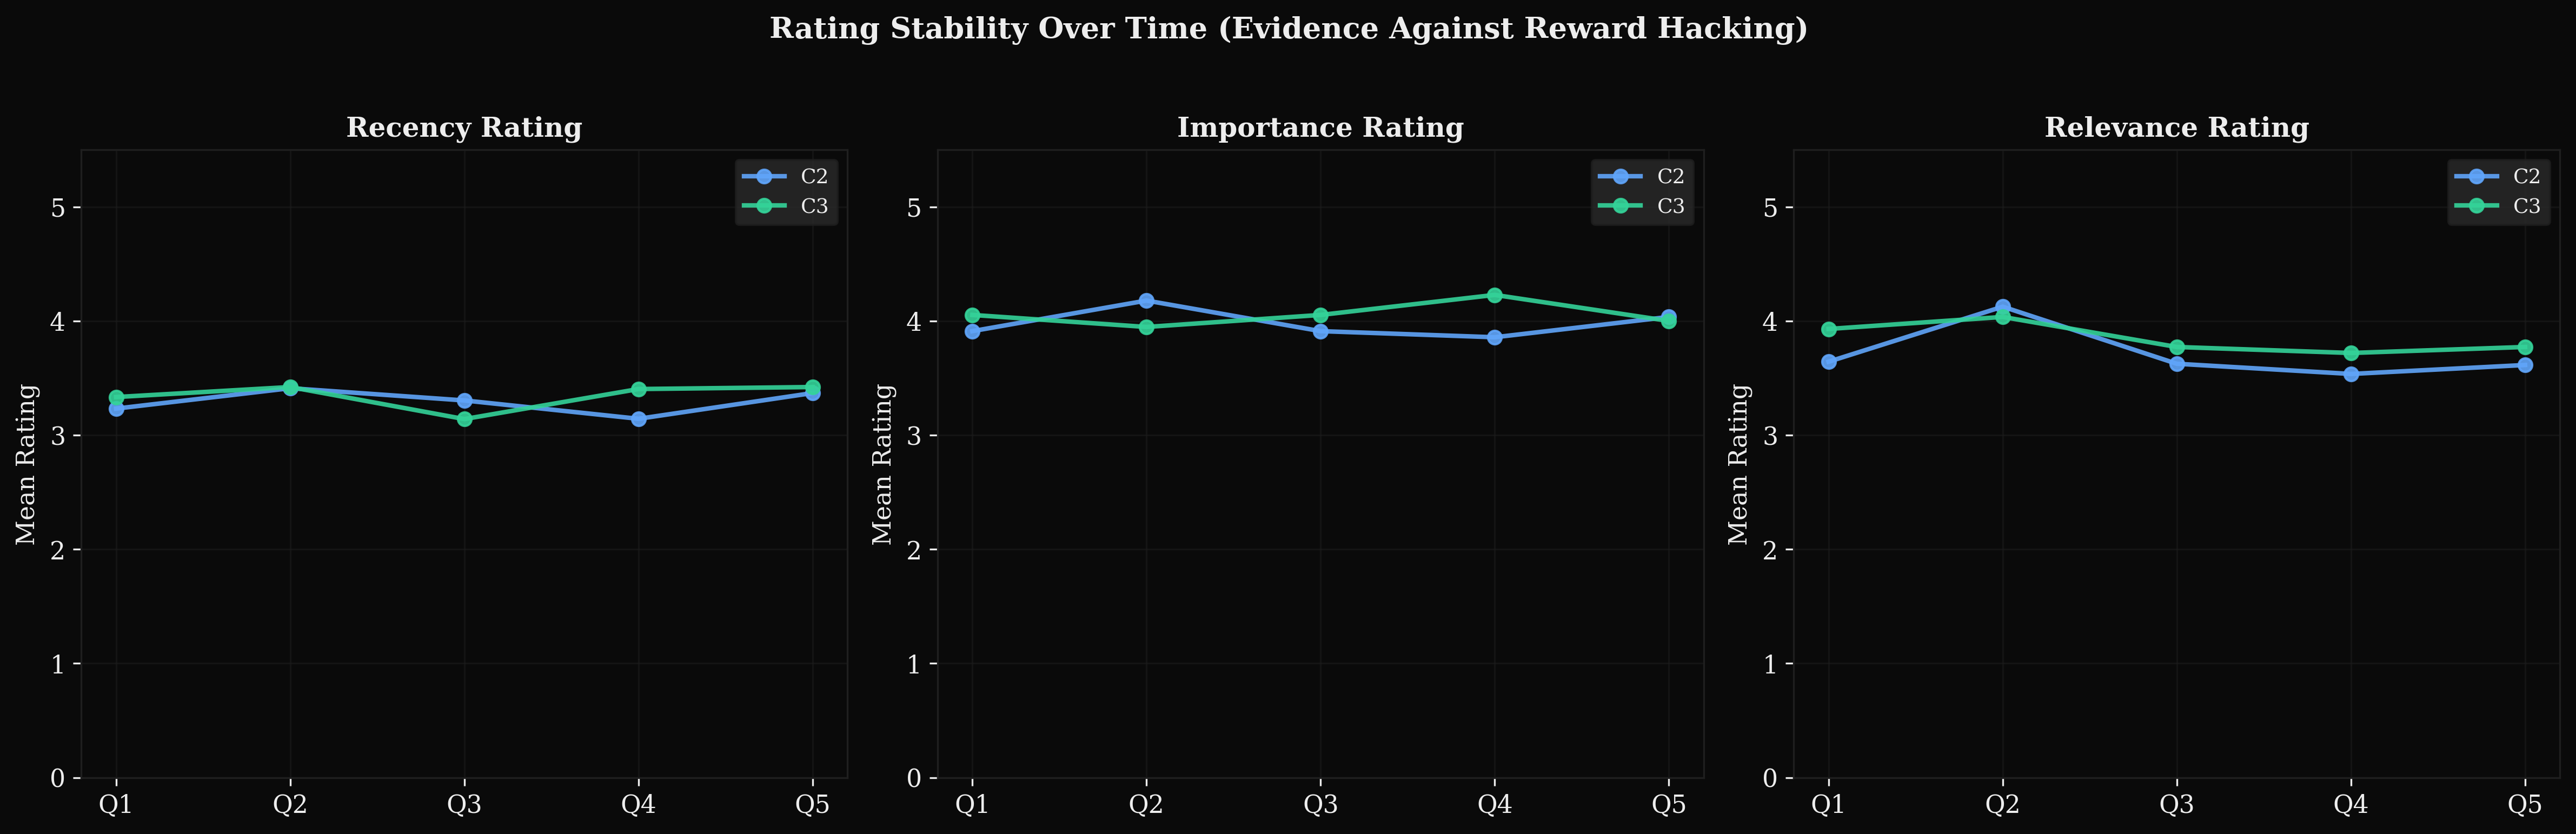
\includegraphics[width=\columnwidth]{../results/figures/figA6_rating_stability.png}
\caption{Dimension rating distributions across quartiles (first 25\%, last 25\% of episodes). Distributions are statistically indistinguishable ($p > 0.3$, KS test), confirming the absence of reward drift or in-context reward hacking.}
\label{fig:rating_stability}
\end{figure}

